\documentclass[11pt, a4paper]{article}

\usepackage[utf8]{inputenc}
\usepackage{fullpage}
\usepackage[parfill]{parskip} % Empty line instead of indentation
\usepackage{graphicx}
\graphicspath{ {images/} }
\usepackage{tabularx}
\usepackage{listings}
\usepackage{caption}
\usepackage{subcaption}
\usepackage{mathtools}
\usepackage{amssymb}
\usepackage{eurosym}
\usepackage[ngerman]{babel}
\usepackage[normalem]{ulem} %Squiggly underline
\usepackage{cancel} %Kürzen

\newcommand\braces[1]{\left(#1\right)}
\newcommand\brackets[1]{\left[#1\right]}
\renewcommand{\vec}[1]{\underline{#1}}
\newcommand{\mat}[1]{\underline{\underline{#1}}}
%\newcommand{\abs}[1]{\left\lvert#1\right\rvert}
\newcommand{\abs}[1]{\left\lvert#1\right\rvert}
%\newcommand{\norm}[1]{\left\lVert#1\right\rVert}
\newcommand{\norm}[1]{\left\lVert#1\right\rVert}
\newcommand\tr[1]{\mathrm{tr}\br{#1}}
\newcommand\average[1]{\left\langle#1\right\rangle}
%\newcommand{\acos}[1]{\mathrm{acos}\braces{#1}}
\newcommand{\acos}{\mathrm{acos}}
%\newcommand{\asin}[1]{\mathrm{asin}\braces{#1}}
\newcommand{\asin}{\mathrm{asin}}
\newcommand{\intend}[1][]{\ \mathrm{d}#1}
\newcommand{\derivative}[2][]{\ \frac{\mathrm{d}#1}{\mathrm{d}#2}} %\derivative[a]{b}
\newcommand\expectedValue[1]{\mathbb{E}\braces{#1}}
\newcommand\variance[1]{\mathbb{V}\braces{#1}}
\newcommand\setequal{\overset{!}{=}}
\newcommand{\gerquote}[1]{\glqq#1\grqq}

%\everymath{\displaystyle} %Force displaystyle everywhere

\lstset{
	tabsize=4,
	breaklines=true,
	showspaces=false
}

\title{Tutorium WS 15/16 \\ Aufgaben}
\author{Christian Mielers}
\date{\today}

\begin{document}
\maketitle
\tableofcontents

\newpage
\section{Höhere Mathematik}
\subsection{Wahrheitstabellen}
Prüfe, ob folgende Aussagen gelten
\begin{enumerate}
	\item $(a \lor b) \lor (a \land b) \Leftrightarrow (a \lor b)$
	\item $(a \lor b) \land (a \lor \lnot b) \Leftrightarrow a \lor (b \land \lnot a)$
	\item $\big((a \lor b) \Rightarrow (a \land b) \big) \Leftrightarrow (a \land b) \lor (\lnot a \land \lnot b)$
\end{enumerate}

\subsection{Mengenlehre}
Gelten die folgenden Beziehungen für beliebige Mengen X, Y und Z?
\begin{enumerate}
	\item $X \setminus (Y \cap Z) = (X \setminus Y) \cap (X \setminus Z)$ %False
	\item $(X \cup Y) \setminus Z = \big((X \setminus Z) \cup (Y \setminus Z)\big) \setminus (Y \cap Z)$ %True
	\item $X \cup (Y \cap Z) = (X \cup Y) \cap (X \cup Z)$ %True
\end{enumerate}

\subsection{Abbildungen}
Sind die folgenden Funktionen injektiv, surjektiv, bijektiv?
\begin{enumerate}
	\item $\mathrm{f}(x) = x^4+2 \qquad \mathrm{f}: \mathrm{R} \mapsto \mathrm{R}$
	\item $\mathrm{f}(x) = x^4+2 \qquad \mathrm{f}: \mathrm{R} \mapsto (2, + \infty)$
	\item $\mathrm{f}(x) = x^3+1 \qquad \mathrm{f}: \mathrm{R} \mapsto \mathrm{R}$
	\item $\mathrm{f}(x) = \sin(x) \qquad \mathrm{f}: \mathrm{R} \mapsto [-1, 1]$
	\item $\mathrm{f}(x) = x^4 - x^2 \qquad \mathrm{f}: \mathrm{R} \mapsto \mathrm{R}$
	\item $\mathrm{f}(x) = \frac{1}{x} \qquad \mathrm{f}: \mathrm{R} \mapsto \mathrm{R}$
\end{enumerate}
Invertiere folgende Funktionen
\begin{enumerate}
	\item $\mathrm{f}(x) = x^3 \qquad \mathrm{f}: \mathrm{R} \mapsto \mathrm{R}$
	\item $\mathrm{f}(x) = \frac{1}{x} \qquad \mathrm{f}: \mathrm{R} \setminus \{0\} \mapsto \mathrm{R} \setminus \{0\}$
	\item $\mathrm{f}(x) =
		\begin{cases}
			- \frac{1}{2}x + 3 & x \in (-\infty, 4) \\
			- 3x + 13 & x \in [4, +\infty)
		\end{cases}
		$
\end{enumerate}

\subsection{Algebraische Strukturen}
Eine Algebraische Struktur kann (u.A.) folgende Eigenschaften aufweisen:
\begin{description}
	\item[A1] Assoziativität (Addition)
	\item[A2] Kommutativität (Addition)
	\item[A3] Neutrales Element (Addition)
	\item[A4] Inverses Element (Addition)
	\item[M1] Assoziativität (Multiplikation)
	\item[M2] Kommutativität (Multiplikation)
	\item[M3] Neutrales Element (Multiplikation)
	\item[M4] Inverses Element (Multiplikation)
	\item[D] Distributivität
\end{description}
Sind A1 - A4 erfüllt handelt es sich um eine Kommutative Gruppe, bei A1-M2 und D um einen Kommutativen Ring und ein Körper ist die Struktur dann, wenn alle Eigenschaften erfüllt sind.

Sind folgende Mengen-Abbildungspaare Gruppen, Ringe, Körper oder nichts davon?
\begin{enumerate}
	\item $\left( \mathbb{N}_0, + \right)$
	\item $\left( \mathbb{Z}, + \right)$
	\item $\left( \mathbb{Z}, +, \cdot \right)$
	\item $\left( \mathbb{R}, +, \cdot \right)$
	\item $\left( \mathrm{M}, +, \cdot \right)$ mit $\mathrm{M} = \{ -2,0,\frac{1
	}{2},1,2 \}$
	\item $\left( \mathbb{R}, +, \circ \right)$ mit $a \circ b = 3a + b$
\end{enumerate}

\subsubsection{Kommutative Gruppen}
Zeige, dass $(G,\circ)$ mit $G=\mathbb{R} \setminus \{1\}$ und $x \circ y = x+y-xy$ eine kommutative Gruppe ist. Was ist das neutrale Element, und wie bildet sich das inverse Element?

\subsubsection{Körper}
Vervollständige folgende Tabellen für den Körper $K = \left\{\{0,1,a,b,c\right\}, +, \cdot\} $. 0 ist das neutrale Element der Addition, 1 der Multiplikation
\begin{center}
	\begin{tabular}{c|ccccc}
		+ & 0 & 1 & a & b & c \\ \hline
		0 &  &  &  &  & \\
		1 &  &  &  &  & \\
		a &  &  &  &  & \\
		b &  &  &  &  & \\
		c &  & 0 & 1 &  & \\
	\end{tabular}
	\hspace{2cm}
	\begin{tabular}{c|ccccc}
		$\cdot$ & 0 & 1 & a & b & c \\ \hline
		0 &  &  &  &  & \\
		1 &  &  &  &  & \\
		a &  &  &  &  & \\
		b &  &  &  &  & \\
		c &  &  &  &  & \\
	\end{tabular}
\end{center}
Was ist das inverse Element von b in K bzgl. der Multiplikation?

\begin{center}
	\begin{tabular}{c|ccccc}
		+ & 0 & 1 & a & b & c \\ \hline
		0 &  &  &  &  & \\
		1 &  &  &  &  & \\
		a &  & 0 & c &  & \\
		b &  &  &  &  & \\
		c &  &  &  &  & \\
	\end{tabular}
	\hspace{2cm}
	\begin{tabular}{c|ccccc}
		$\cdot$ & 0 & 1 & a & b & c \\ \hline
		0 &  &  &  &  & \\
		1 &  &  &  &  & \\
		a &  &  &  &  & \\
		b &  &  &  &  & \\
		c &  &  &  &  & \\
	\end{tabular}
\end{center}

\subsection{Summen und Produkte}
Berechne folgende Summen:
\begin{enumerate}
	\item $\sum_{k=2}^{15} 4$
	\item $\sum_{k=0}^5 k^3$
	\item $\sum_{k=0}^5 (-1)^k (4k+3)$
\end{enumerate}
Berechne folgende Produkte:
\begin{enumerate}
	\item $\prod_{i=1}^7 i$
	\item $\prod_{i=1}^4 \frac{i}{2}$
	\item $\prod_{i=1}^4 \frac{3j^2+2}{j}$
\end{enumerate}

\subsection{Binomialkoeffizient}
Für den Binomialkoeffizienten gilt:
$\binom{n}{k} = \frac{n!}{k!(n-k)!}$ \qquad $\binom{n}{n-k} = \binom{n}{k}$ (Symmetrie)

Welchen Wert hat $n$ in den folgenden Gleichungen?
\begin{enumerate}
	\item $ n = \binom{6}{3}$
	\item $n = \binom{10}{7}$
	\item $\binom{n+3}{n+1} + \binom{n+4}{n+2} + \binom{n-1}{n-3} = 70$
\end{enumerate}

\subsection{Ordnungsrelationen}
Ergänze bei folgenden Ausdrücken die Relationszeichen $\subset, \subseteq, \supseteq, \supset,$ \\
\begin{tabular}{|l|c|l|}
	\hline
	Menge 1 & \hspace{3mm} ? \hspace{3mm} & Menge 2 \\ \hline
	$\{1,2,3\}$ & & $\{1,2,3\}$ \\
	$\{5,6\}$ & & $\{5,6,7,8\}$ \\
	$\{\sqrt{2}, \pi, 3\}$ & & $\mathbb{R}$ \\
	$\mathbb{R}$ & & $\mathbb{Q} \setminus {\pi, e}$ \\
	$\mathbb{N}_0$ & & $\mathbb{N}$ \\
	$\mathbb{I}$ & & $\mathbb{R}$ \\
	$\mathbb{C} \setminus \mathbb{I}$ & & $\mathbb{Q} \setminus \mathbb{N} \cup \{2,4,6\}$ \\ \hline
\end{tabular}

\subsection{Ungleichungen}
Für welche Werte von $x$ gelten die folgenden Ungleichungen?
\begin{enumerate}
	\item $5x-3 < \dfrac{2x^2+3x}{x}$
	\item $\dfrac{x+1}{2} \geq \abs{2x-3}$
	\item $\sqrt{x^2-2x+1} > 3 - |x-2|$
	\item $\sqrt{x^2-8x+16} < \frac{\abs{x+2}}{2}$
	\item $\sqrt{x^2-2x+1} > 3 + |x-2|$
\end{enumerate}

\subsection{Induktion}
Beweise per vollständiger Induktion:
\begin{enumerate}
	\item $\forall n \geq 1 : \sum_{i=1}^n i = \dfrac{n(n+1)}{2}$
	\item $\forall n \geq 1 : \sum_{i=1}^n (2i-1) = n^2$
	\item $\forall n \geq 1 : \sum_{i=1}^n (2i-1)^2 = \frac{n (2n-1)(2n+1)}{3}$
	\item $\forall n \geq 1 : \quad 3 \mid (n^3 - n)$
	\item $\forall n \geq 4 : \quad 2^n \geq n^2$
\end{enumerate}

\subsection{Einheitskreis}
\begin{figure}[h!]
	\centering
	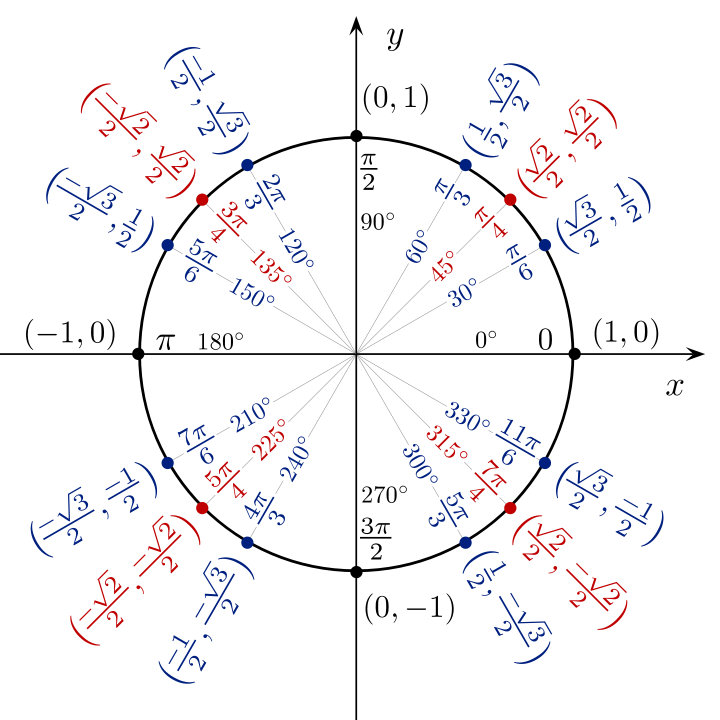
\includegraphics[width=0.5\textwidth]{Einheitskreis.png}
	\caption{Einheitskreis: (cos, sin)}
	\label{einheitskreis}
\end{figure}

Lese aus dem Einheitskreis (Abbildung \ref{einheitskreis}) ab:
\begin{enumerate}
	\item $\cos \frac{\pi}{4}$
	\item $\sin \frac{5\pi}{4}$
	\item $\acos -\frac{\sqrt{3}}{2}$
	\item $\asin -\frac{1}{2}$
\end{enumerate}

\subsection{Komplexe Zahlen}
Gegeben seien folgende Zahlen aus $\mathbb{C}$. Bestimme den Real- und Imaginärteil, die komplex konjugierte so wie den Betrag:
\begin{enumerate}
	\item $2i - (2 + i) + (7 - 4i)$
	\item $(1-i)^2$
	\item $\frac{3 - i}{2 + 2i}$
	\item $(2 - i) + (3 + i)(3-i)$
	\item $i^{\ 2015}$
\end{enumerate}

\subsubsection{Polarkoordinaten und Exponentialdarstellung}
Schreibe als Polarkoordinaten- und Exponentialdarstellung \\
Polarkoordinaten: $r(\cos \alpha + i \sin \alpha)$ mit $r=\sqrt{x^2+y^2}$ und $\acos \frac{x}{r} = \alpha = \asin \frac{y}{r}$
\begin{enumerate}
	\item $\sqrt{2}+\sqrt{2}i$
	\item $-4i$
	\item $6+2\sqrt{3}i$
\end{enumerate}
Schreibe als Summe von Real- und Imaginärteil \\
Karthesische Darstellung: x + yi
\begin{enumerate}
	\item $7 \left( \cos \pi + i \sin \pi \right)$
	\item $\sqrt{3} \left( \cos \frac{\pi}{3} + i \sin \frac{\pi}{3} \right)$
	\item $2 \cdot e^{i \frac{5 \pi}{3}}$
\end{enumerate}

\subsubsection{Rechnen in Polarkoordinaten}
Für 2 komplexe Zahlen $z_1$, $z_2$ mit Polarkoordinatendarstellung $z_i = r_i \braces{\cos \alpha_i + i \sin \alpha_i}$ gilt:

$z_1 \cdot z_2 = r_1 r_2 \braces{ \cos \braces{\alpha_1 + \alpha_2} + i \sin \braces{\alpha_1 + \alpha_2}}$ \\
$z_1 \div z_2 = \frac{r_1}{r_2} \braces{\cos \braces{\alpha_1 - \alpha_2} + i \sin \braces{\alpha_1 - \alpha_2}}$ \\
$z_1^n = r_1^n \braces{\cos (n \alpha_1) + i \sin (n \alpha_1)}$ \\
$\sqrt[n]{z_1} = w_k$ mit $w_k = \sqrt[n]{r_1} \braces{\cos \frac{\alpha_1 + 2k\pi}{n} + i \sin \frac{\alpha_1 + 2k\pi}{n}}, k = 0, \dots n-1$

Berechne in Polarkoordinaten:
\begin{enumerate}
	\item $3 \left( \cos \frac{2\pi}{3} + i \sin \frac{2\pi}{3} \right) \cdot \sqrt{4} \left( \cos \pi + i \sin \pi \right)$
	\item $4 \left( \cos \frac{7\pi}{6} + i \sin \frac{7\pi}{6} \right) \div 2 \left( \cos \pi + i \sin \pi \right)$
	\item $\left( 3+\sqrt{3}i \right)^4$
	%TODO weitere Aufgabe zum Potenzieren und Wurzelziehen (mit besseren Zahlen)
	\item $p^4 + 16 = 0$
\end{enumerate}

\subsection{Folgen}
\subsubsection{DGL}
\begin{description}
	\item[Folgen 1. Ordnung] $a_{n+1} = q \cdot a_n + d$
		\begin{align*}
			a_n = \begin{cases}
				a_0 \cdot q^n + d \cdot \frac{1-q^n}{1-q}, &\text{ falls } q \in \mathbb{R} \setminus \{1\} \\
				a_0 + d \cdot n &\text{ falls } q=1
					\end{cases}
		\end{align*}
	\item[Folgen 2. Ordnung] $a_{n+1} = b a_n + c a_{n-1}$ \vspace{0.3cm} \\
		Für das charakteristisches Polynom $q^2 = bq+c$ mit Nullstellen $q_1, q_2$ gibt die folgende Tablle in Abhängigkeit davon, ob bei der PQ-Formel der Teil unter der Wurzel positiv, $0$ oder negativ ist, die explizite Form an.
		
		\begin{tabular}{|c|l|}
			\hline
			Diskriminante & Explizite Darstellung \\ \hline
			$>0$ & $a_n = C_1 q_1^n + C_2 q_2^n$ \\
			$=0$ & $a_n = C_1 q_1^n + C_2 n \cdot q_2^n$ \\
			$<0$ & $a_n = C_1 r^n \cos(n\alpha) + C_2 r^n \sin(n\alpha)$ \\ \hline
		\end{tabular}
\end{description}

Finde die explizite Darstellung von $a_n$. Gib auch den Grenzwert $\lim_{n \rightarrow \infty} a_n$ an.
\begin{enumerate}
	\item $a_{n+1} = 3 a_n + 6$ mit $n \in \mathbb{N}, a_0 = 4$
	\item $a_{n+1} = 2 a_n +2$ mit $n \in \mathbb{N}_0,\ a_1 = 4$
	\item $a_{n+2} = 5 a_{n+1} - 3$ mit $n \in \mathbb{N}, a_0 = 1$
	\item $a_{n+1} = -6 a_{n} - 5 a_{n-1}$ mit $a_0=2, a_1=4$
	\item $a_{n+1} = 3 a_n - 4 a_{n-1}$ mit $a_0=3, a_1=4$
\end{enumerate}

\subsection{Reihen}
\subsubsection{Konvergenz und Divergenz}
Konvergieren die folgenden Reihen?
\begin{enumerate}
	\item $\sum_{k=0}^\infty \frac{(2k+2)(3k-2)}{(2k-2)^2}$
	\item $\sum_{k=0}^\infty \frac{(k-1)^2}{\sqrt{3^k}}$
	\item $\sum_{k=2}^\infty \frac{\sqrt{2k-1}}{k^2-k+\frac{1}{4}}$
\end{enumerate}

\subsubsection{Grenzwerte}
Konvergieren die folgenden Reihen? Wenn ja, berechne auch den Grenzwert:
\begin{enumerate}
	\item $\sum_{k=4}^\infty \frac{1}{k^2-5k+6}$
	\item $\sum_{k=0}^\infty \frac{2}{k^2+6k+8}$
	\item $\sum_{k=0}^\infty \frac{(-1)^k \cdot 2^{k-1} - 5 \cdot 6^k}{4^{2k+1}}$
\end{enumerate}

\subsection{Logarithmen}
Löse die folgenden Gleichungen:
\begin{enumerate}
	\item $\frac{1}{2} \log x + \log \sqrt{x-1} = \log \sqrt{2}$
	\item $\log_{10} \left( 15 \cdot 50^x + 2 \cdot 2^x \right) = \log_{10} 15 + x$
\end{enumerate}

\subsection{Analysis}
\subsubsection{Partialbruchzerlegung}
Berechne mittels Partialbruchzerlegung:
\begin{enumerate}
	\item $\int_4^6 \frac{3x}{x^2 - 2x - 3} dx$ %(x+1)(x-3)
	\item $\int_2^3 \frac{x-1}{x^3 + 4x^2 + 5x + 2} dx$ %(x+1)^2(x+2)
\end{enumerate}

\subsubsection{Substitution}
\[ \int_a^b \mathrm{f}( \ \underbrace{\mathrm{g}(x)}_t \ ) \intend{x} = \int_{\mathrm{g}(a)}^{\mathrm{g(b)}} \mathrm{f}(t) \intend{t} \]
Berechne mittels Substitution:
\begin{enumerate}
	\item $\int_{-\pi}^\pi \sin{x} \cdot \cos{x} \intend{x}$
	\item $\int_1^e \frac{\sqrt{\ln(x)}}{x} \intend{x}$
	\item $\int_\frac{\pi}{2}^\pi e^{3 \cos x} \cdot \sin x \intend{x}$
\end{enumerate}

\subsubsection{Partielle Integration}
\[ \int \mathrm{f}(x) \ \mathrm{g}'(x) \intend{x} = \left[ \mathrm{f}(x) \ \mathrm{g}(x) \right] - \int \mathrm{f}'(x) \ \mathrm{g}(x) \intend{x} \]
Berechne mittels partieller Integration:
\begin{enumerate}
	\item $\int_0^1 3x^2 e^x \intend{x}$
\end{enumerate}

\newpage
\section{Statistik}
\subsection{Klassische Wahrscheinlichkeitsrechnung}
\subsubsection{Würfel}
Ein fairer Würfel wird geworfen. Wie groß ist die Wahrscheinlichkeit, dass \dots
\begin{enumerate}
	\item eine 3 geworfen wird?
	\item eine 3 oder eine 4 geworfen wird?
	\item eine Primzahl $> 3$ geworfen wird?
	\item eine Primzahl oder eine Zahl $> 3$ geworfen wird?
\end{enumerate}
Nun wird mit 2 Würfeln geworden. Wie groß ist die Wahrscheinlichkeit, dass \dots
\begin{enumerate}
	\item die Augensumme 7 ist?
	\item die Augensumme durch 4 teilbar ist?
\end{enumerate}

\subsubsection{Das Urnenmodell}
\begin{tabular}{|c|c|c|}
	\hline
	\multicolumn{3}{|c|}{Aus Menge mit \textbf{n} Elementen \textbf{k} ziehen} \\
	\hline
	 & \textbf{mit} Beachtung der Reihenfolge & \textbf{ohne} Beachtung der Reihenfolge \\
	\hline
	\textbf{mit} Zurücklegen & $n^k$ & $\dbinom{n+k-1}{k} = \dfrac{(n+k-1)!}{k!\cdot (n-1)!}$ \\
	\hline
	\textbf{ohne} Zurücklegen & $\dfrac{n!}{(n-k)!}$ & $\dbinom{n}{k} = \dfrac{n!}{k!\cdot (n-k)!}$ \\
	\hline
\end{tabular}

In einer Urne liegen 12 Kugeln: 9 blaue und 3 rote. Aus dieser ziehen wir 3 Kugeln. Wie groß ist dann die Wahrscheinlichkeit (mit/ohne) Zurücklegen und (mit/ohne) Reihenfolge, dass \dots
\begin{enumerate}
	\item alle Kugeln blau sind?
	\item zwei blaue und eine rote Kugeln gezogen werden?
	\item höchstens eine rote Kugel gezogen wird?
\end{enumerate}

\subsection{Bedingte Wahrscheinlichkeit}
Der \textit{TIOBE-Index} misst die Verbreitung verschiedener Programmiersprachen, z.B. auf Basis von öffentlichen Repositories (Quellcode-Speicherorte). Aktuell (Januar 2014) gilt unter den Top4 folgende Aufteilung (gerundet, sonstige nicht betrachtet, C++ gefittet):
\begin{description}
	\item[C] 37\%
	\item[Java] 31\%
	\item[Objective-C] 19\%
	\item[C++] 13\%
\end{description}
Ab hier wird es fiktiv: 63\% aller Programme werden unter Windows entwickelt. Von allen C++-Programmen werden 67\% unter Windows geschrieben, von den Java-Programmen sind es 93\%. Von den reinen C-Programmen werden 41\% unter sonstigen Betriebsystemen entwickelt. \\
\\
Gib eine vollständige Wahrscheinlichkeitstabelle an (auf 2 Nachkommastellen runden).

\subsection{Statistische Abhängigkeit}
Prof. Müller liest die Vorlesung Thermodynamik zwei mal in der Woche, Montags um 8:30 und Donnerstags um 12:00. Er glaubt, dass sich Montags morgens wesentlich weniger Studenten aufraffen können zur Vorlesung zu kommen, und außerdem, dass bei Regen die Hörerzahlen ebenfalls zurück gehen. Darum hat er die Wahrscheinlichkeiten für die drei Ereignisse \emph{Wenig Hörer (W)}, \emph{Morgens (M)} und \emph{Regen (R)} und ihre Kombinationen in einer Tabelle festgehalten: \\

\begin{tabular}{c|c|c|c|c|c|c|c}
	Normal & W & M & R & WM & WR & MR & WMR \\ \hline
	0.25 & 0.05 & 0.2 & 0.08 & 0.402 & 0.002 & 0.015 & 0.002
\end{tabular} \\
\\
Hängt die Hörerzahl tatsächlich von der Uhrzeit bzw. vom Regen ab?

\subsection{Zufallsvariablen}
Für die \emph{ganzzahlige} Zufallsvariable X seien folgende Wahrscheinlichkeiten bekannt, Werte $X > 4$ gibt es nicht:
\begin{itemize}
	\item $W(X == 0) = 0.2$
	\item $W(X == 2) = 0.2$
	\item $W(X \leq 3) = 0.8$
	\item $W(X > 1) = 0.4$
\end{itemize}
Gib die Wahrscheinlichkeits- und die Verteilungsfunktion an.

\newpage
\section{Informatik}
\subsection{Variablen und Zuweisungen}
Schreibe ein Programm, dass die Daten zu einem Auto auf der Konsole ausgibt. Das Auto hat folgende Daten:
\begin{description}
	\item[Hersteller] Audi
	\item[Modell] A8
	\item[Beschleunigung] 4.1 m/s
	\item[Gewicht] 2000 kg
\end{description}
\begin{enumerate}
	\item Beginne damit, die notwendigen Variablen zu deklarieren
	\item Weise den Variablen nun die passenden Werte zu
	\item Gib außerdem die vom Auto entwickelte Kraft an \\
	(Erinnerung aus der Physik: $\vec{F}=m\vec{a}$, Kraft = Masse $\cdot$ Beschleunigung)
\end{enumerate}

\subsection{Bedingte Ausführung}
Es soll ein Login erstellt werden, bei dem ein Nutzer seinen Namen und sein Passwort eingeben muss. Das Programm soll dann ausgeben, ob die eingegebenen Daten akzeptiert werden oder nicht. Gültige Login-Daten sind:
\begin{itemize}
	\item Name: Balzebub, Passwort: Meisterklasse1337
	\item Name: foo, Passwort: bar
\end{itemize}
Nutze für die Namen eine Switch- und für die Passwörter eine if-Abfrage.
\paragraph{Tipp} Zwei Strings können im if folgendermaßen auf Gleichheit geprüft werden:
\begin{lstlisting}[language=Java, tabsize=4]
	string1.equals(string2)
\end{lstlisting}

\subsection{Schleifen}
Es soll ein Rätsel programmiert werden, bei dem der Computer eine Zufallszahl zwischen 1 und 100 generiert und der Nutzer diese erraten muss. Das Programm sagt einem dabei, ob die geratene Zahl zu groß, zu klein oder genau richtig ist.
\begin{enumerate}
	\item Ist sie richtig, beendet sich das Programm, ansonsten läuft es weiter.
	\item Erweitere das Programm anschließend so, dass der Benutzer maximal 8 Versuche hat. Die Zahl des Versuchs soll mit ausgegeben werden.
\end{enumerate}
\paragraph{Tipp} Eine Zufallszahl zwischen 1 und 100 kann erzeugt werden mit:
\begin{lstlisting}[language=Java]
	Random generator = new Random();
	int geheim = generator.nextInt(100) + 1;
\end{lstlisting}

\subsection{Rekursion}
Ein Sonnensystem hat P Planeten, die allesammt bewohnt sind. Der innerste Planet hat eine Einwohnerzahl von $E_1$, der zweite hat die hälfte davon, der dritte wiederrum die hälfte vom zweiten Planeten usw.
\begin{enumerate}
	\item Schreibe eine rekursive Funktion, die die Einwohnerzahl des p-ten Planeten ausrechnet.
	\item Wie viele Einwohner $E_{13}$ hat der 13. Planet, wenn der innerste Planet 16 Milliarden und 384 Millionen ($16.384.000.000$) Einwohner hat?
\end{enumerate}
\paragraph{Tipp} \texttt{int} hat einen Wertebereich von $-2^{31}$ bis $2^{31}-1$. Das entspricht etwa $-2$ Milliarden bis $+2$ Milliarden.
\paragraph{Anmerkung} Es handelt sich hierbei um eine Folge, man könnte die Einwohnerzahl von Planet p auch direkt ausrechnen mit: $E_1 \cdot \left(\frac{1}{2}\right)^{p-1}$

\newpage
\section{Programmieren in C}
\subsection{Syntax}
Schreibe das obligatorische \texttt{Hello World} Programm. Wie sieht der Funktionskopf der Main-Methode aus? Welche Methode ermöglicht die Ausgabe?

\subsection{Altersabfrage}
Ein Programm soll das Alter von Personen überprüfen. Dazu geben sie ihr Geburtsjahr ein (der Einfachheit halber betrachten wir nicht das genaue Datum). Das Programm gibt dann aus, ob sie jünger oder älter sind als 18.

\paragraph{Tipp} Um das aktuelle Jahr zu ermitteln, kann folgende Funktion verwendet werden, die das Einbinden von time.h erfordert und das Jahr als Integer zurück gibt.
\begin{lstlisting}[language=C]
	#include <time.h>

	int getYear() {
		time_t t = time(NULL);
		struct tm *lTime = localtime(&t);
		return lTime->tm_year + 1900;
	}
\end{lstlisting}

\subsection{Strings}
Gegeben sei folgender Test:
\begin{quote}
	N'Gasta! Kvata! Kvakis! ahkstas so novajxletero (oix jhemile) so Ranetauw. Ricevas gxin pagintaj membrauw kaj aliaj individuauw, kiujn iamaniere tusxas so raneta aktivado. En gxi aperas informauw unuavice pri so lokauw so cxiumonataj kunvenauw, sed nature ankoix pri aliaj aktuasoj aktivecauw so societo. Ne malofte enahkstas krome plej diversaspekta materialo eduka oix distra.
\end{quote}
\begin{enumerate}
	\item Nimm an, der Text liegt als \texttt{cstring (char array)} vor. Gib den Text und die Anzahl Zeichen des Textes aus.
	\item Das Programm soll nun jedes Vorkommen des \textbf{Wortes} \glqq so\grqq\ durch \glqq AI\grqq\ ersetzen (wenn die Zeichenfolge \glqq so\grqq\ innerhalb eines anderen Wortes vorkommt, soll sie nicht verändert werden). Gib den neuen Text und seine Länge aus. Erkläre ggf. das Ergebnis.
	\item Gib die Position aus, an der das erste \glqq AI\grqq\ im neuen Text beginnt.
	\item Wie lang ist nun der ursprüngliche Text? Erkläre ggf. das Ergebnis.
\end{enumerate}

\subsection{Input, Output}
%TODO Fragen "Nerds, what is your profession?"
%AI! AI! AI! eingeben lassen
%Ausgeben, ob die Antwort richtig war
%Nenne es GeistiBlockPlus, Adblock logo

\subsection{Zeiger 1}
Im folgenden Programm sollen die Werte der Variablen \texttt{number1} und \texttt{number2} getauscht werden. Welche der \texttt{swap}-Funktionen leisten dies?
\lstinputlisting[language=C]{src/zeigerVariablenTauschen.c}

\subsection{Zeiger 2}
\label{zeigerAufgabe}
Schreibe eine Funktion, die ein Array und seine Länge übergeben bekommt. Die Funktion soll das Minimum und das Maxium zurück geben. Das Array hat den Datentyp \texttt{short}.

Wende die Funktion auf das folgende Array an:
7, 4, 1, 5, 9, 4

\subsection{Const Correctness}
Das Keyword \texttt{const} dient dazu, Variablen als Konstant zu deklarieren, sie dürfen vom Programmierer also nicht verändert werden. Ergänze das Programm aus \ref{zeigerAufgabe} um \texttt{const}-Markierungen, wo es möglich ist. Was bewirkt es an den jeweiligen Stellen?

\newpage
\section{Wirtschaftlichkeitsanalyse}
\subsection{Grundbegriffe}
Ordne die Vorgänge dem jeweiligen Begriff zu. Eine Abrechnungsperiode entspricht einem Monat.

\begin{tabularx}{\columnwidth}{X|c|c|c|c}
	Vorgang & Auszahlung & Ausgabe & Aufwand & Kosten \\ \hline
	Der Lieferdienst bringt eine Couch vorbei. Wir zahlen bar. &   &   &  &  \\ \hline
	Bestellung eines Handwerkers, er kommt nächsten Monat. Wir werden bar zahlen. &  &  &  &  \\ \hline
	Überweisung von 30 \euro \ für einen Laserpointer, der letzten Monat ankam. &   &  &  & \\ \hline
	Wir essen 5 Tiefkühlpizzen, die unser Nachbar letzten Monat vorbei gebracht hat. Wir geben ihm dafür einen Fünfer. &   &  &   &  
\end{tabularx}

\subsection{Kapitalwert}
Dem Karnevalsverein B.W.L (Bochumer Weißwurst Liga) steht durch den Abbau seiner Niederlassung in Querenburg die Summe von 300'\euro \ zur Verfügung, die langfristig investiert werden soll. Dafür hat sie folgende Optionen:
\begin{enumerate}
	\item Anheuern der talentierten Büttenrednerin Berta Wassermann. Diese erklärt sich bereit, für 200' \euro \ die nächsten 3 Jahre auf Prunksitzungen des Vereins aufzutreten. Der Verein erwartet dadurch zusätzliche Einnahmen von 120' \euro \ pro Jahr.
	\item Investition in Ü-Ei Sammelfiguren. Auf einer bekannten online Autionsbörse steht zur Zeit eine Sammlung von zehntausend Figuren im Gesammtwert von 220' \euro \ zum Verkauf. Diese generieren keinen Mehrwert, aber der Marketingleiter der B.W.L geht davon aus, die Figuren in 4 Jahren für 480' \euro \ verkaufen zu können.
	\item Anlage bei einer Bank. Da der Filialleiter auch gleichzeitig Prinz des Karnevalsumzugs ist, gibt es hier Zinsen von 10\%.
\end{enumerate}
Berechne den Kapitalwert der Anlagen. Für welche sollte sich B.W.L entscheiden?

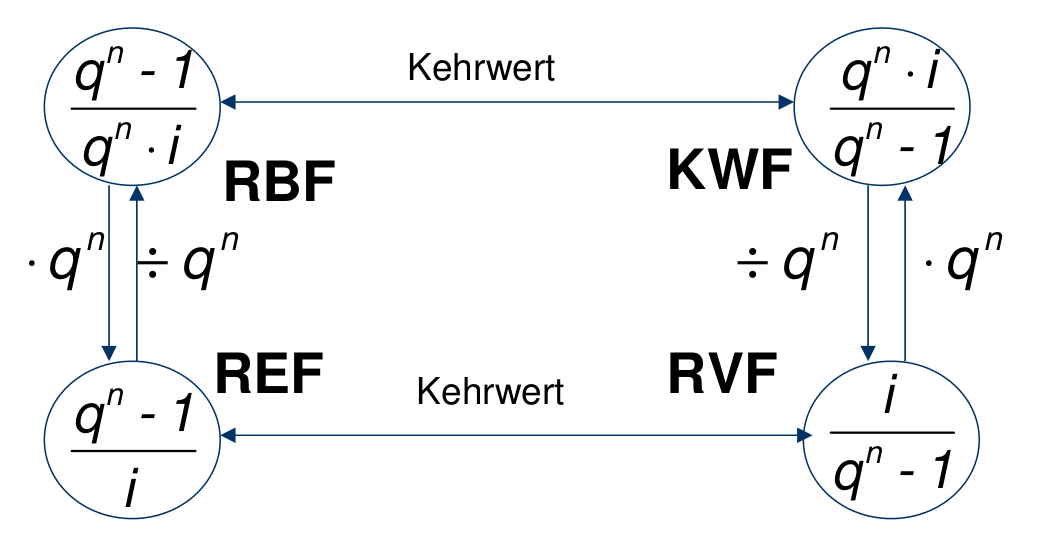
\includegraphics[height=4cm]{RentenUndKapitalfaktoren.png}

\subsection{Investitionsrechnung}
Helmut B. plant die Eröffnung einer Druckerei. Dafür ist die Anschaffung einer Buchpresse erforderlich. Nachdem er Angebote eingeholt hat, stehen folgende Pressen, die jeweils 5 Jahre genutzt werden sollen, in der engeren Auswahl:

\vspace{\baselineskip}
\begin{tabular}{l|r|r}
	& Presse 1 & Presse 2 \\ \hline
	Anschaffungskosten (\euro) & 450.000 & 300.000 \\
	sonstige fixe Kosten (\euro) p.a. & 15.000 & 12.000 \\
	variable Kosten (\euro \ pro Verpackungseinheit) & 22 & 25 \\
	Restverkaufserlös (\euro) & 80.000 & 50.000
\end{tabular}

\vspace{\baselineskip}
Herr B. geht davon aus, 14.000 Verpackungseinheiten mit jeweils 20 Büchern verkaufen zu können und rechnet mit 5\% Zinsen.

\begin{enumerate}
	\item Welche Presse ist nach Kostenvergleichsrechnung die bessere Wahl?
	\item Bei welcher Produktionsmenge an Verpackungseinheiten sind beide Pressen gleich gut?
	\item Da Presse 1 zusätzlich noch das Gesicht des Charmanten Herrn B. auf das Cover drucken kann, rechnet her hier mit einem Verkaufspreis von 18\euro \ je Buch, bei Presse 2 jedoch nur mit 16\euro \ je Buch. Für welche Presse entscheidet er sich nach einer Gewinnvergleichsrechnung? Wir nehmen dabei an, dass Presse 1 Kosten von 410.000 \euro \ und Presse 2 Kosten von 420.000 \euro \ verursacht (Vermeidung von Folgefehlern).
\end{enumerate}

\subsection{Äquivalenzziffernrechnung}
Der Lebensmittelhersteller Krafft vertreibt 4 Sorten Energy-Drinks. Die Kosten pro Palette ergeben sich zum Großteil aus der Herstellungsdauer. In der folgenden Tabelle sind die Herstellungszahlen und Produktionszeiten pro Palette und Typ angegeben. Die gesammten Herstellungskosten betragen 320.000 \euro.

\begin{tabular}{lcc}
	Energy-Drink & Produktionszahlen (in Paletten) & Hertellungsdauer (in Minuten) \\ \hline
	Ungehäuer & 2400 & 24 \\
	Blue Donkey & 1200 & 32 \\
	Rhinozeros & 600 & 18 \\
	Rockikone & 2000 & 20
\end{tabular}

\vspace{\baselineskip}
Wie groß sind die Herstellungskosten in vollen Tausend \euro \ pro Produkttyp, wenn man die einstufige Äquivalenzziffernrechnung anwendet?

\newpage
\section{Sonstiges}
\subsection{Binäre Zahlen}
Welche Dezimalzahlen entsprechen den folgenden Binärzahlen?
\begin{enumerate}
	\item 110, 1010, 10001
	\item 11101, 100100, 1110001101
\end{enumerate}
Welche Binärzahlen entsprechen den folgenden Dezimalzahlen?
\begin{enumerate}
	\item 1, 2, 4, 8, 16
	\item 3, 7, 15
	\item 5, 11, 28, 42
\end{enumerate}
Führe folgende Berechnungen durch
\begin{enumerate}
	\item $1101_b + 110_b$
	\item $1011101_b + 1001_b$
	\item $1011101_b - 1001_b$
	\item $1101_b - 110_b$
	\item $1101_b \cdot 110_b$
	\item $1011101_b \cdot 1001_b$
\end{enumerate}

\subsection{Modulare Arithmetik}
Was ist das Ergebnis folgender Rechnungen?
\begin{enumerate}
	\item $3 \bmod 3 \equiv \text{?}$
	\item $7 \bmod 3 \equiv \text{?}$
	\item $13 \bmod 5 \equiv \text{?}$
\end{enumerate}
Wozu sind die folgenden Terme äquivalent?
\begin{enumerate}
	\item $3 + 4 \pmod 2$
	\item $12 + 1 \pmod 5$
	\item $4 \cdot 5 \pmod 7$
	\item $3 \cdot 8 \pmod {11}$
\end{enumerate}
Welches x löst die Gleichung?
\begin{enumerate}
	\item $0 + x \equiv 3 \pmod 5$
	\item $1 + x \equiv 0 \pmod 5$
	\item $4 + x \equiv 2 \pmod 5$
\end{enumerate}

\subsection{Versionsverwaltung mit Git}

\end{document}









